\documentclass{beamer}
\usepackage{beamerthemeshadow}
\usepackage{xmpmulti}
\usefonttheme[onlymath]{serif}


\graphicspath{ {./graphics/} }

\usecolortheme{rose}
\usetheme{Warsaw}


\title{Petaluma High School}
\author{Mr. Kelley}
\institute{Petaluma High School}
\date{Fall 2012}


\newcommand{\m}{\mbox{ m }}
\newcommand{\kg}{\mbox{ kg }}
\newcommand{\s}{\mbox{ s }}
\newcommand{\ke}{\mbox{\small KE}}
\newcommand{\pe}{\mbox{\small PE}}


\newcommand{ \bigLPic}[2]{
       \includegraphics[scale = .34]<#1>{#2}}

\newcommand{ \bigPPic}[2]{
       \includegraphics[angle = -90, scale = .20]<#1>{#2}}

\newcommand{ \halfnhalfLR}[2]{
       \begin{columns}
       \column{.5\textwidth}
       #1
       \column{.5\textwidth}
       #2
       \end{columns}
}
\newcommand{ \halfnhalfBR}[2]{
       \begin{columns}
       \column{.3\textwidth}
       #1
       \column{.7\textwidth}
       #2
       \end{columns}
}

\newcommand{ \halfnhalfBL}[2]{
       \begin{columns}
       \column{.7\textwidth}
       #1
       \column{.3\textwidth}
       #2
       \end{columns}
}

\newcommand{ \halfnhalfRL}[2]{
       \begin{columns}
       \column{.5\textwidth}
       #2
       \column{.5\textwidth}
       #1
       \end{columns}
}



\begin{document}

\section{Universal Gravitation}

\frame{
	\frametitle{Universal Gravitation}
	\mbox{} 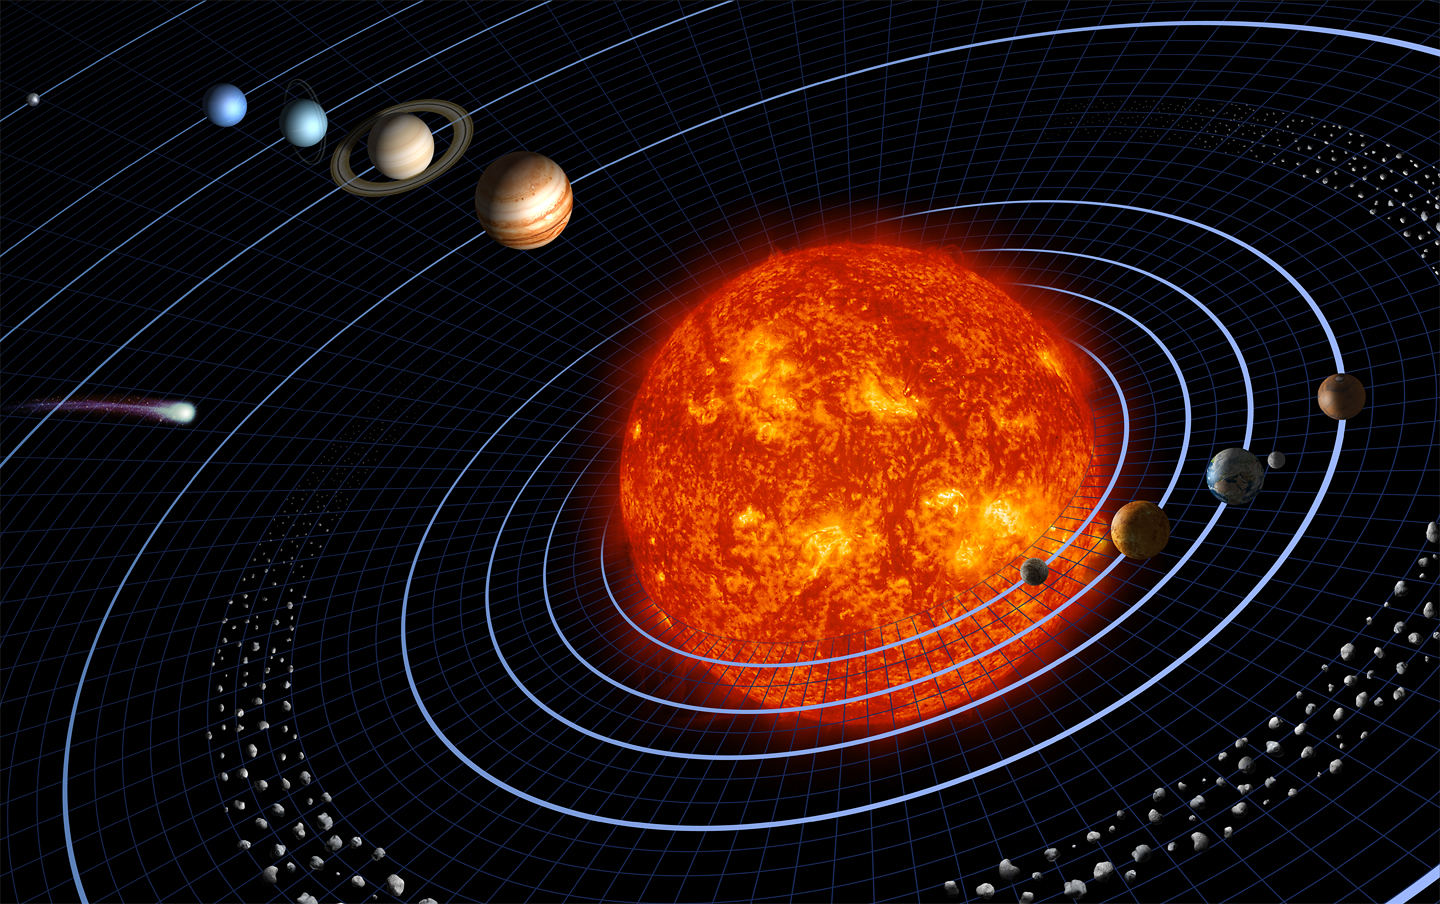
\includegraphics[scale = .2]{solarSys.jpg} \hfill \mbox{}
	}

\frame{
	\frametitle{Satellite Motion}
	How fast does a Volkswagon Beetle have to be moving in order to sustain an orbit a mere 1 km above the surface of the earth?  What about 200 km above the surface?
	}
	
\frame{
	\frametitle{Energy Review}
	
	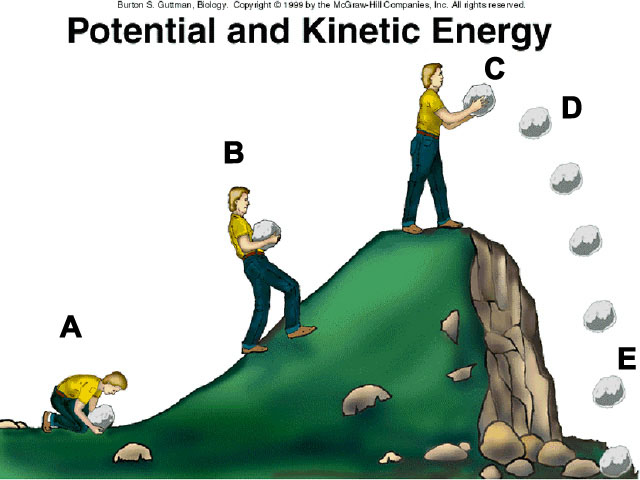
\includegraphics[scale = .45]{rockEnergy.jpg} \\ 
	}

\frame{
       \frametitle{Energy Review}
       
	\halfnhalfLR{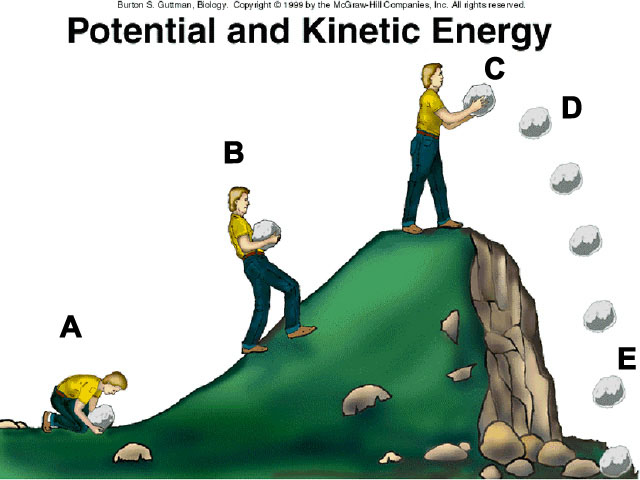
\includegraphics[scale = .25]{rockEnergy.jpg}}{
	\begin{itemize}
	\pause
	\item Where does the total energy of the rock equal {\bf zero}? \pause
	\item Where does the rock have the greatest {\bf potential} energy? \pause
	\item Where does the rock have the greatest {\bf kinetic} energy? \pause
	\item If the rock started at `A' with zero energy, and ended up at `E' with non-zero energy, {\bf where} did that energy come from? \pause
	\item Where is there {\bf work} being done on the rock?
	\end{itemize}
	%\raisebox{4cm}{This is called the Work Energy Theorem}
	}
}

\frame{
	\frametitle{Potential Energy}
	
	\begin{center}
	Remember Baumgartner's big jump?  It was from 39 km above the surface of the earth.  Calculate $\Delta \pe$ using
	\end{center}
	\uncover<2>{$$\pe = mgh$$}
	\uncover<3->{$$U = -G \frac{m_1 m_2}{r}$$} \\
	\vspace{.5cm}
	\uncover<4->{What does it mean if $U=0$?}  \uncover<5>{How far away is that?}
}

\frame{
	\frametitle{Projectiles, Again}
	\centering
If we launch a projectile at the surface of the earth, it will follow a predictable path. \\ \vfill 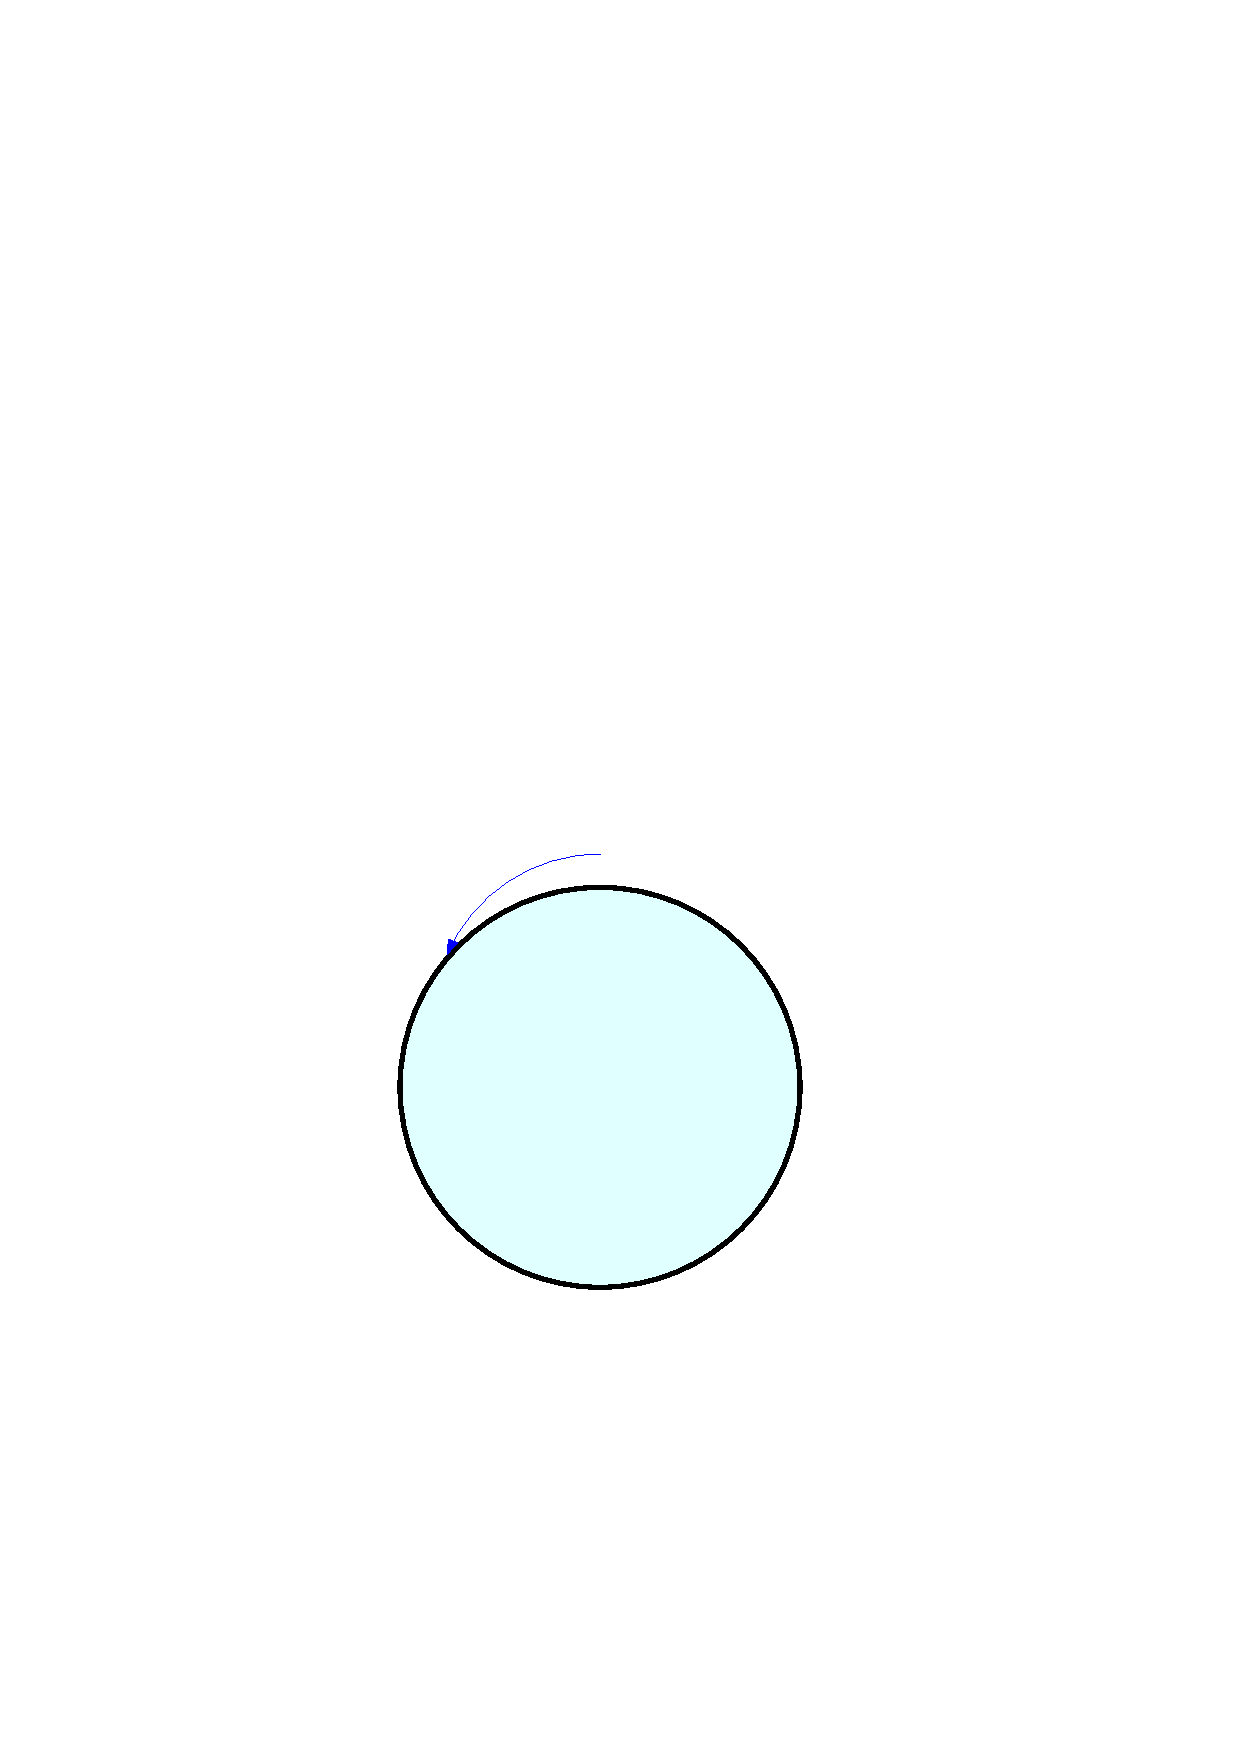
\includegraphics[scale = .7]{ballistic1}
}
\frame{
	\frametitle{Projectiles, Again}
	\centering
If we launch a projectile hard enough, it will follow a different kind of predictable path. \\ \vfill 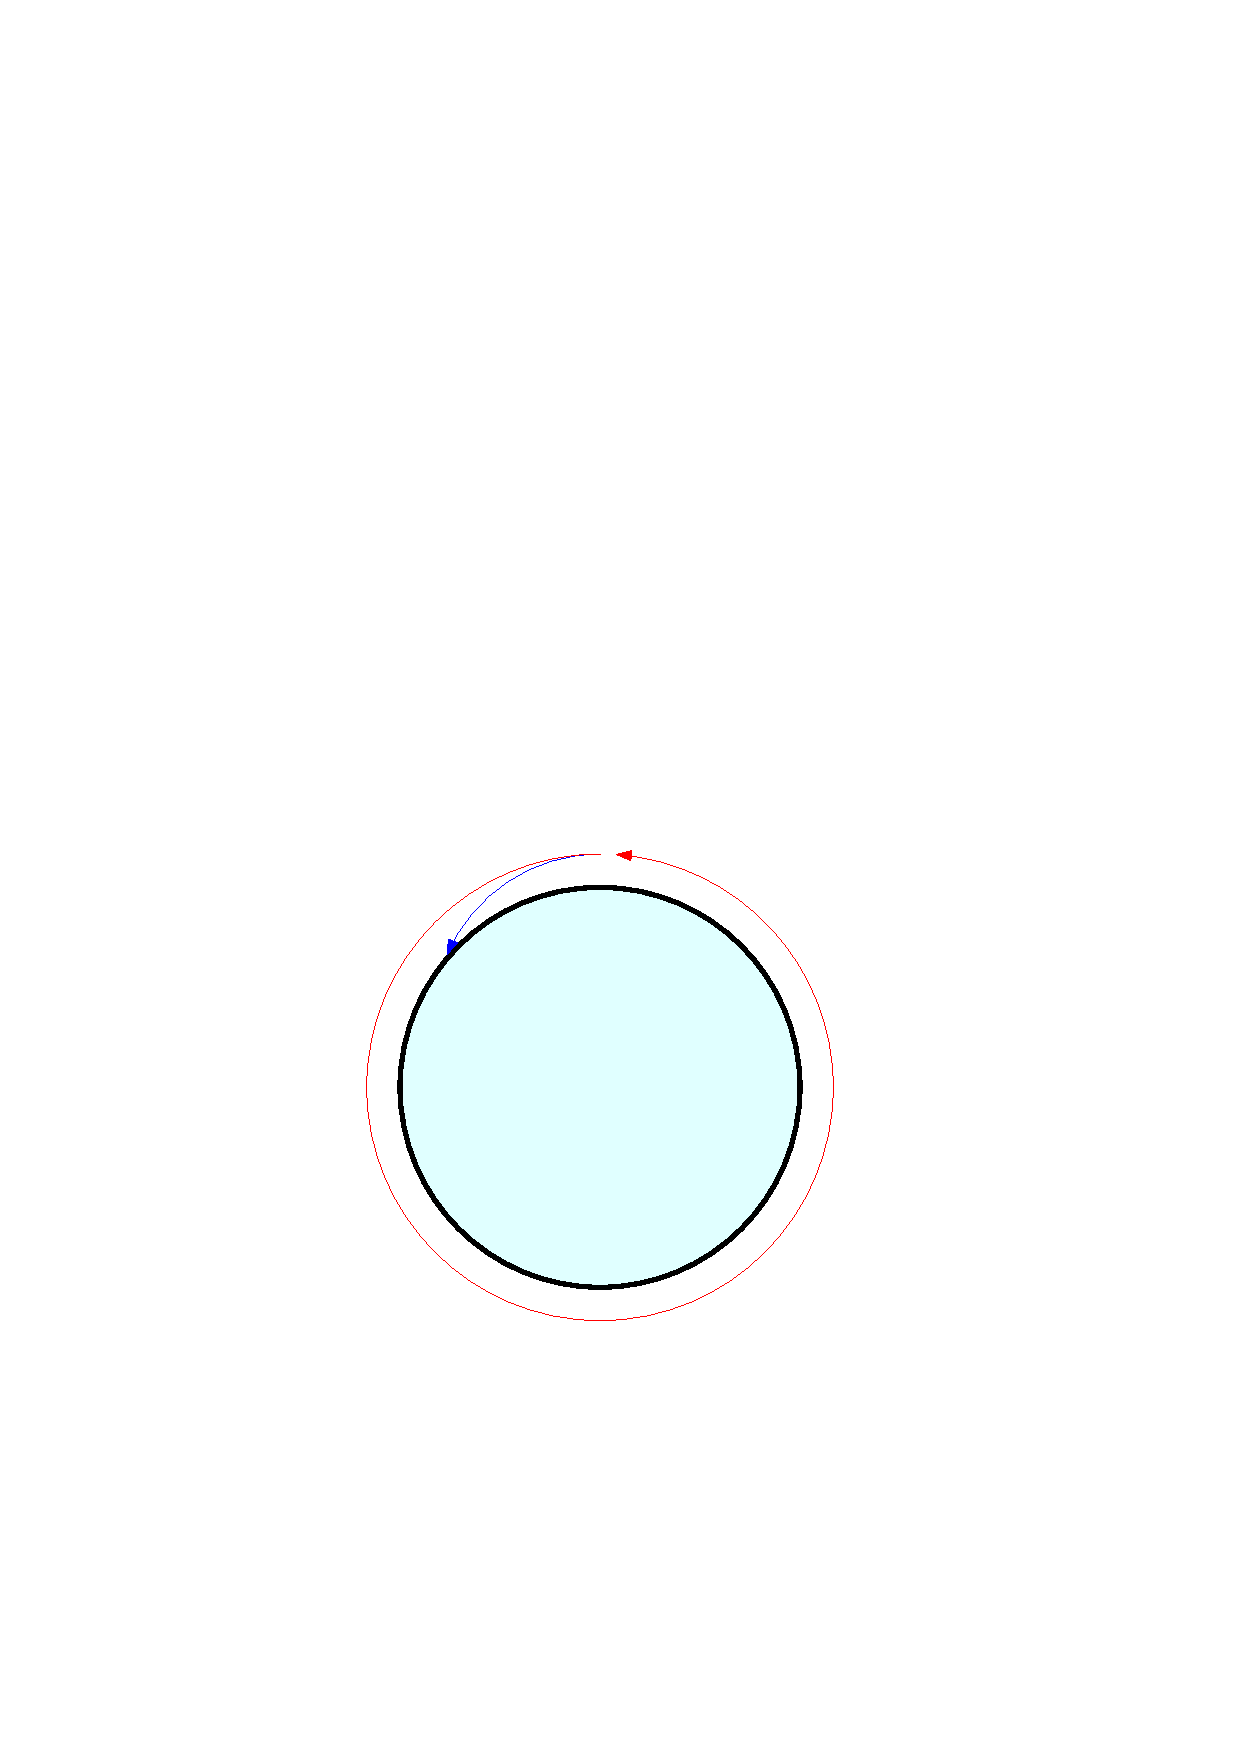
\includegraphics[scale = .7]{ballistic2}
}
\frame{
	\frametitle{Projectiles, Again}
	\centering
Satellites can also assume elliptical orbits. \\ \vfill 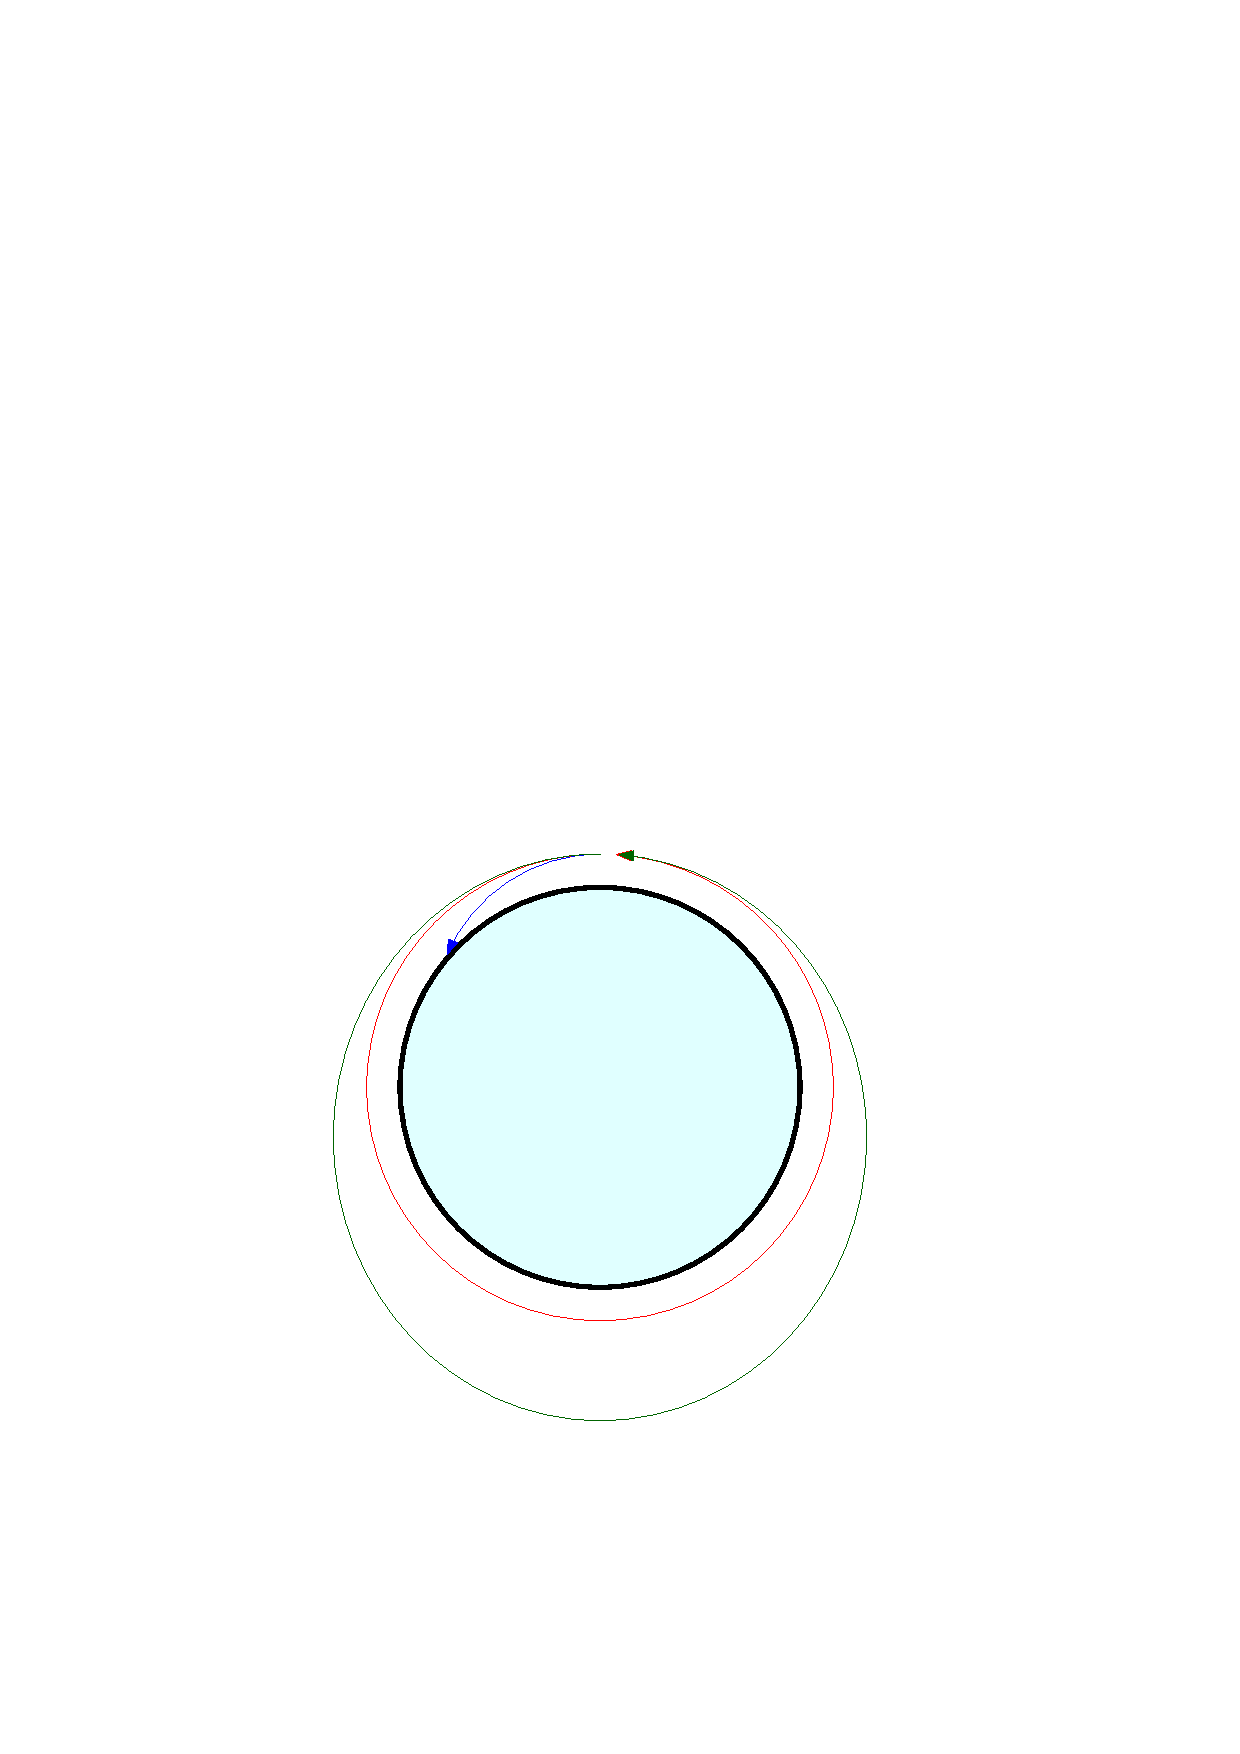
\includegraphics[scale = .7]{ballistic3}
}
\frame{
	\frametitle{Projectiles, Again}
	\centering
If we launched something hard enough, it would never come back, nor would it assume an orbit \\ \vfill 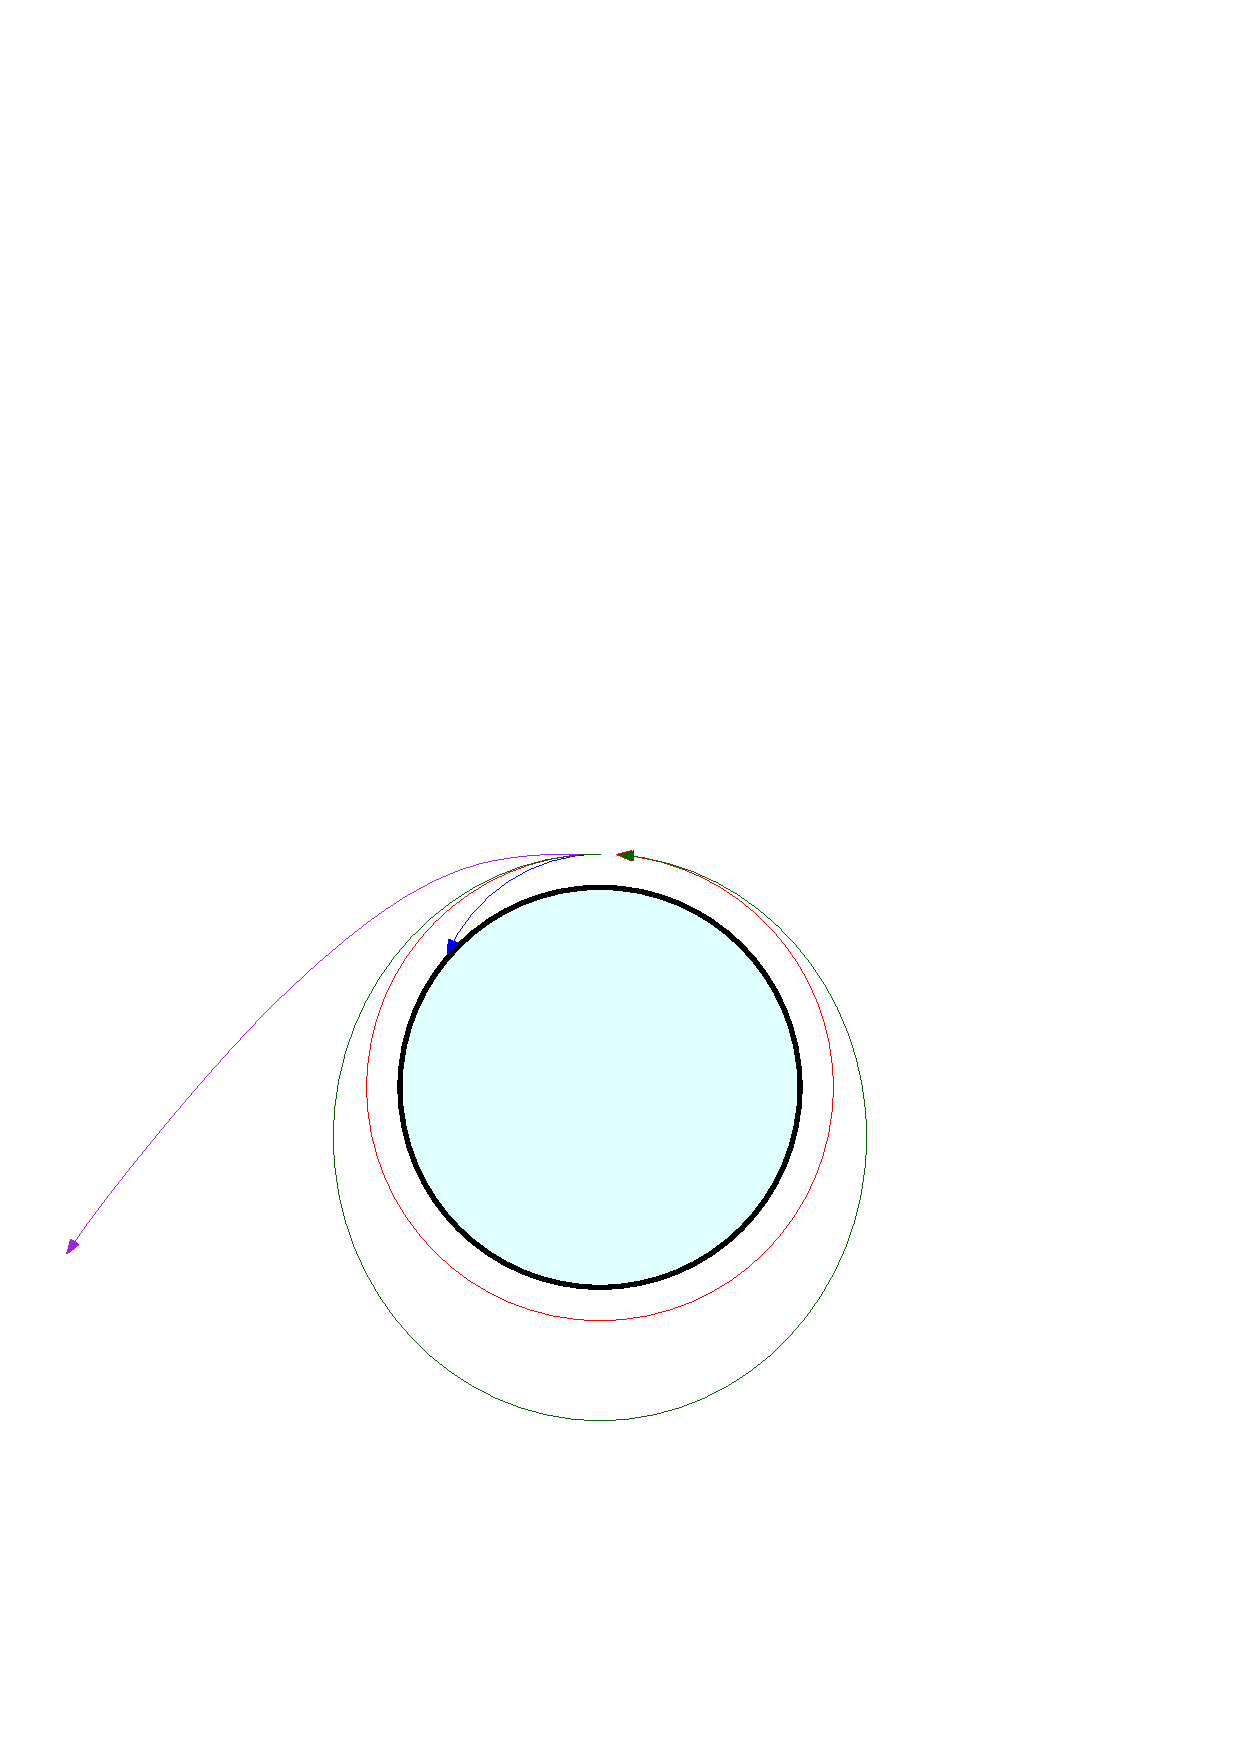
\includegraphics[scale = .7]{ballistic4}
	
     }

\frame{
	\frametitle{Escape Velocity}
	
	\centering
	So how hard would we have to launch an object for it to escape the gravitational pull of the earth? \\ \pause \vspace{1cm}
	Consider the familiar equation stating conservation of mechanical energy:
	$$\ke_\circ + \pe_\circ = \ke_f +\pe_f$$ \pause
	Or using $U$:
	$$\ke_\circ + U_\circ = \ke_f +U_f$$
	
     }

\frame{
	\frametitle{Escape Velocity}
	
	\begin{align*}
	\ke_\circ + U_\circ &= \ke_f +U_f \\ \\
	\vspace{1cm}
	\frac{1}{2} m_1 v_\circ^2 - G \frac{m_1 m_2}{r_\circ} &= 0 + 0
	\end{align*}
	$$v_e = \sqrt{\frac{2Gm}{r}}$$
     }




\frame{
	\frametitle{Black Holes}
	\centering
	To approximate black hole physics, we can consider a body with an escape velocity greater than or equal to the speed of light.
	$$c = 3.0 \times 10^8 \mbox{ m/s}$$
     }

\frame{
	\frametitle{Black Holes}
	
	What is the \emph{event horizon} of a black hole with 11 times the mass of our sun?
	
     }

\end{document}